\documentclass{extbook}[14pt]
\usepackage{multicol, enumerate, enumitem, hyperref, color, soul, setspace, parskip, fancyhdr, amssymb, amsthm, amsmath, bbm, latexsym, units, mathtools}
\everymath{\displaystyle}
\usepackage[headsep=0.5cm,headheight=0cm, left=1 in,right= 1 in,top= 1 in,bottom= 1 in]{geometry}
\pagestyle{fancy}
\lhead{}
\chead{Answer Key for Module\,6\,-\,Polynomial\,Functions Version C}
\rhead{}
\lfoot{Summer\,C\,2020}
\cfoot{}
\rfoot{}
\begin{document}
\textbf{This key should allow you to understand why you choose the option you did (beyond just getting a question right or wrong). \href{https://xronos.clas.ufl.edu/mac1105spring2020/courseDescriptionAndMisc/Exams/LearningFromResults}{More instructions on how to use this key can be found here}.}

\textbf{If you have a suggestion to make the keys better, \href{https://forms.gle/CZkbZmPbC9XALEE88}{please fill out the short survey here}.}

\textit{Note: This key is auto-generated and may contain issues and/or errors. The keys are reviewed after each exam to ensure grading is done accurately. If there are issues (like duplicate options), they are noted in the offline gradebook. The keys are a work-in-progress to give students as many resources to improve as possible.}

\rule{\textwidth}{0.4pt}

26. Construct the lowest-degree polynomial given the zeros below. Then, choose the intervals that contain the coefficients of the polynomial in the form $x^3+bx^2+cx+d$.
\[ 4 - 5i \text{ and } 1 \] 
The solution is $ x^{3} -9 x^{2} +49 x -41 $ 

\begin{enumerate}[label=\Alph*.] 
\item $ b \in [5, 18], c \in [42, 60], \text{ and } d \in [39, 50] $ 

 $x^{3} +9 x^{2} +49 x + 41$, which corresponds to multiplying out $(x-(4 - 5i))(x-(4 + 5i))(x + 1)$. 
\item $ b \in [-4, 6], c \in [-3, 7], \text{ and } d \in [-11, 1] $ 

 $x^{3} + x^{2} +4 x -5$, which corresponds to multiplying out $(x + 5)(x -1)$. 
\item $ b \in [-12, 0], c \in [42, 60], \text{ and } d \in [-50, -33] $ 

 * $x^{3} -9 x^{2} +49 x -41$, which is the correct option. 
\item $ b \in [-4, 6], c \in [-9, 0], \text{ and } d \in [3, 5] $ 

 $x^{3} + x^{2} -5 x + 4$, which corresponds to multiplying out $(x -4)(x -1)$. 
\item $ \text{None of the above.} $ 

 This corresponds to making an unanticipated error or not understanding how to use nonreal complex numbers to create the lowest-degree polynomial. If you chose this and are not sure what you did wrong, please contact the coordinator for help. 
\end{enumerate} 
 
General Comments: Remember that the conjugate of $a+bi$ is $a-bi$. Since these zeros always come in pairs, we need to multiply out $(x-(4 - 5i))(x-(4 + 5i))(x-(1))$.

-----------------------------------------------

27. Which of the following equations \textit{could} be of the graph presented below?
\begin{center} 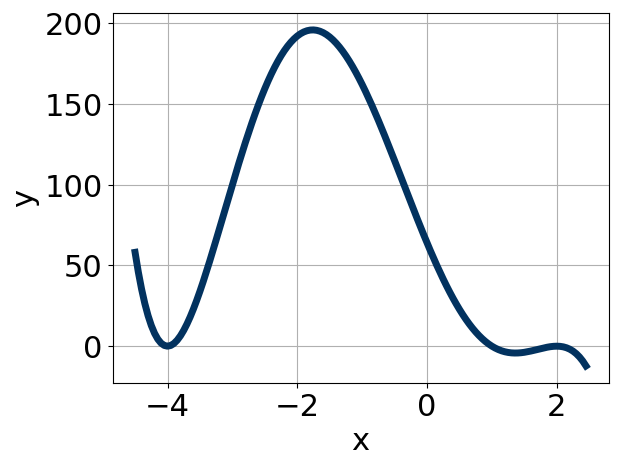
\includegraphics[width=0.3\textwidth]{../Figures/polyGraphToFunctionC.png} \end{center} 

The solution is $ -12(x + 1)^{6} (x - 2)^{6} (x - 3)^{11} $ 

\begin{enumerate}[label=\Alph*.] 
\item $ -8(x + 1)^{6} (x - 2)^{5} (x - 3)^{9} $ 

 The factor $(x - 2)$ should have an even power. 
\item $ -18(x + 1)^{8} (x - 2)^{5} (x - 3)^{6} $ 

 The factor $(x - 2)$ should have an even power and the factor $(x - 3)$ should have an odd power. 
\item $ 4(x + 1)^{6} (x - 2)^{10} (x - 3)^{8} $ 

 The factor $(x - 3)$ should have an odd power and the leading coefficient should be the opposite sign. 
\item $ 18(x + 1)^{4} (x - 2)^{10} (x - 3)^{11} $ 

 This corresponds to the leading coefficient being the opposite value than it should be. 
\item $ -12(x + 1)^{6} (x - 2)^{6} (x - 3)^{11} $ 

 * This is the correct option. 
\end{enumerate} 
 
General Comments: Draw the x-axis to determine which zeros are touching (and so have even multiplicity) or cross (and have odd multiplicity).

-----------------------------------------------

28. Construct the lowest-degree polynomial given the zeros below. Then, choose the intervals that contain the coefficients of the polynomial in the form $ax^3+bx^2+cx+d$.
\[ \frac{-6}{5}, 3, \text{ and } \frac{7}{5} \] 
The solution is $ 25x^{3} -80 x^{2} -27 x + 126 $ 

\begin{enumerate}[label=\Alph*.] 
\item $ a \in [19, 30], b \in [-150, -138], c \in [231, 241], \text{ and } d \in [-130, -122] $ 

 $25x^{3} -140 x^{2} +237 x -126$, which corresponds to multiplying out $(5x + 5)(x -1)(5x -5)$. 
\item $ a \in [19, 30], b \in [-90, -74], c \in [-32, -21], \text{ and } d \in [123, 132] $ 

 * $25x^{3} -80 x^{2} -27 x + 126$, which is the correct option. 
\item $ a \in [19, 30], b \in [73, 86], c \in [-32, -21], \text{ and } d \in [-130, -122] $ 

 $25x^{3} +80 x^{2} -27 x -126$, which corresponds to multiplying out $(5x -6)(x + 3)(5x + 7)$. 
\item $ a \in [19, 30], b \in [-90, -74], c \in [-32, -21], \text{ and } d \in [-130, -122] $ 

 $25x^{3} -80 x^{2} -27 x -126$, which corresponds to multiplying everything correctly except the constant term. 
\item $ a \in [19, 30], b \in [5, 11], c \in [-159, -150], \text{ and } d \in [123, 132] $ 

 $25x^{3} +10 x^{2} -153 x + 126$, which corresponds to multiplying out $(5x + 5)(x + 1)(5x -5)$. 
\end{enumerate} 
 
General Comments: To construct the lowest-degree polynomial, you want to multiply out $(5x + 6)(x -3)(5x -7)$

-----------------------------------------------

29. Describe the end behavior of the polynomial below.
\[ f(x) = -5(x + 2)^{4}(x - 2)^{5}(x - 6)^{2}(x + 6)^{2} \] 

 
 The solution is  
 \begin{center} 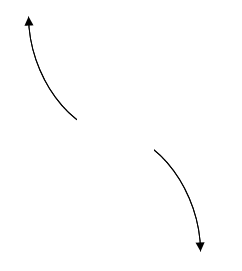
\includegraphics[width=0.3\textwidth]{../Figures/polyEndBehaviorAC.png} \end{center}\begin{tabular}{|c|c|} 
\hline 
 & \tabularnewline 
 \textbf{A.} 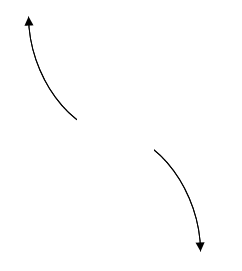
\includegraphics[width=0.3\textwidth]{../Figures/polyEndBehaviorAC.png} & \textbf{B.} 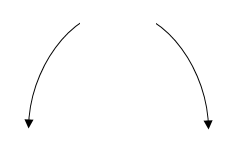
\includegraphics[width=0.3\textwidth]{../Figures/polyEndBehaviorBC.png} \tabularnewline 
\hline 
 & \tabularnewline 
 \textbf{C.} 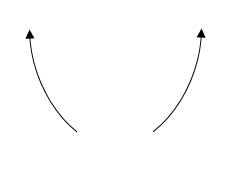
\includegraphics[width=0.3\textwidth]{../Figures/polyEndBehaviorCC.png} & \textbf{D.} 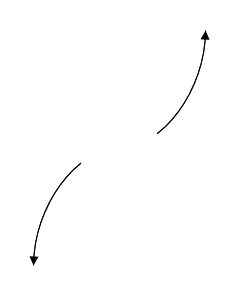
\includegraphics[width=0.3\textwidth]{../Figures/polyEndBehaviorDC.png} \tabularnewline 
\hline 
 E. None of the figures above. & \tabularnewline 
\hline 
 \end{tabular} 
 
\begin{enumerate}[label=\Alph*.] 
\item The function is above the $x$-axis, then passes through.  
\item The function is below the $x$-axis, then touches.  
\item The function is above the $x$-axis, then touches.  
\item The function is below the $x$-axis, then passes through.  
\end{enumerate} 
 
\textbf{General Comments:} Remember that end behavior is determined by the leading coefficient AND whether the \textbf{sum} of the multiplicities is positive or negative.

-----------------------------------------------

30. Describe the zero behavior of the zero $x = 2$ of the polynomial below.
\[ f(x) = -6(x + 4)^{10}(x - 4)^{8}(x - 2)^{11}(x + 2)^{6} \] 

 
 The solution is  
 \begin{center} 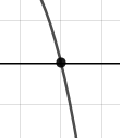
\includegraphics[width=0.3\textwidth]{../Figures/polyZeroBehaviorAC.png} \end{center}\begin{tabular}{|c|c|} 
\hline 
 & \tabularnewline 
 \textbf{A.} 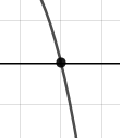
\includegraphics[width=0.3\textwidth]{../Figures/polyZeroBehaviorAC.png} & \textbf{B.} 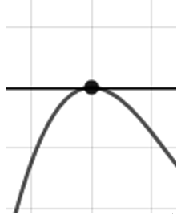
\includegraphics[width=0.3\textwidth]{../Figures/polyZeroBehaviorBC.png} \tabularnewline 
\hline 
 & \tabularnewline 
 \textbf{C.} 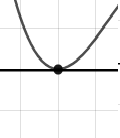
\includegraphics[width=0.3\textwidth]{../Figures/polyZeroBehaviorCC.png} & \textbf{D.} 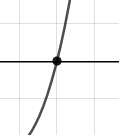
\includegraphics[width=0.3\textwidth]{../Figures/polyZeroBehaviorDC.png} \tabularnewline 
\hline 
 E. None of the figures above. & \tabularnewline 
\hline 
 \end{tabular} 
 
\begin{enumerate}[label=\Alph*.] 
\item   
\item   
\item   
\item   
\end{enumerate} 
 
\textbf{General Comments:} You will need to sketch the entire graph, then zoom in on the zero the question asks about.

-----------------------------------------------


\end{document}

